%
% File naaclhlt2015.tex
%

\documentclass[11pt,letterpaper]{article}
\usepackage{naaclhlt2015}
\usepackage{times}
\usepackage{graphicx}
\usepackage{latexsym}
\usepackage{graphicx}
\setlength\titlebox{6.5cm}    % Expanding the titlebox

\title{Minerva \\ Question-answering system}

\author{Meris Bahtijaragic\\
	    {\tt dat11mba@student.lu.se}
	    \And
      \\
      \\
      \\
      \textbf{Tim Dolck}\\
      {\tt dat11tdo@student.lu.se}
      \And
      Julian Kron\'{e}\\
      {\tt dat11jkr@student.lu.se}
}

\date{}

\begin{document}
\maketitle
\begin{abstract}
In this paper a question answering system including passage retrieval and answer 
extraction is described and evaluated.
The question answering system described is designed for Swedish questions and answers, and 
uses Swedish Wikipedia as its data source. The system is trained using transcribed 
questions from the Swedish board game Kvitt eller dubbelt. These questions are also used 
for testing.

The main tools used when developing the system were Apache Lucene, Stagger and Liblinear.

\end{abstract}
\section{Introduction}
This project is a Swedish question answering system developed in the course EDAN70 at LTH.
The goal is to create a system that is able to answer questions with one word long answers.
To do this, the Swedish Wikipedia were used as data source, and the annotated questions from the Swedish 
board game Kvitt eller dubbelt, transcribed by Juri Pyykk\"o, Rebecka Weegar, Pierre Nugues \cite{QASYS}, was used as training questions and categories. 

A fundamental system overview is shown in figure \ref{fig:overview}. 

\begin{figure*}
\centering
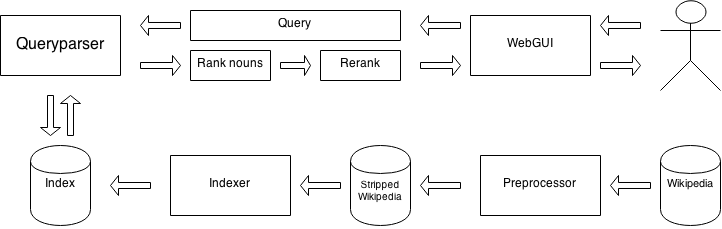
\includegraphics[width=1\textwidth]{figures/Question-answering-system.png}
\caption{Overview}
\label{fig:overview}
\end{figure*}

\section{Question Processing}
\subsection{Preprocessing of questions}
Given a question, the system will first of all convert the question
to a format which can be used to perform a query to the indexed
database. This is done by whitelisting all characters which
are not in our supported swedish alphabet. The question is also
processed through a linear classifier to determine the category of our 
answers.

\subsection{Training the Question Classifier}
For this system, the training data consists of 2300 questions 
from the swedish board game Kvitt eller Dubbelt transcribed 
by Juri Pygg\"o, Rebecka Weegar, Piere Nugues \cite{QASYS}.

The training data consists of 2300 questions containing 9 datafields each.
The system is only concerned with two datafields on each question:
\begin{itemize}
\item Question Formulation - The original question taken from the transcribed
  card.
\item Answer Class - Which was manually determined during transcription. 
  Possible values: concept, location, description, multiplechoice, amount, organization, 
  other, person, abbreviation, verb, title, timepoint, duration, money.
\end{itemize}
After processing the training set using \texttt{libshorttext}, a model file is created.
By using this model file, the system can classify 
what class an answer is expected to have, for example the question \textit{vad heter sveriges huvudstad?} 
yields the following Class-Probability pairs:
\begin{center}
  \begin{tabular} {l c}
    \texttt{location}    & \texttt{1.00} \\
    \texttt{concept}     & \texttt{0.69} \\
    \texttt{verb}        & \texttt{0.63} \\
    \texttt{description} & \texttt{0.52} \\
    \texttt{money}       & \texttt{0.50} \\
  \end{tabular}
\end{center}

\section{Passage Retrieval}
The purpose of the passage retriever is to reduce the information to a size that is more manageable.
Given a question, the passage retriever translates this into a query, and searches the index for passages 
relevant to this query. Where these passages are sorted by their similarity to the query.
The passage retriver is entirely built upon Lucene Core, an open source, Java-based system, 
that is capable of fast and effective indexing, and smart querying.

\subsection{Wikipedia}
As mentioned, the Swedish Wikipedia is used as information source, downloaded from Wikimedia {reference here} as wikitext embedded in XML.
To gather the useful text, a python script was used to simply remove everything but the text. 
This script were slightly modified to accomodate both indexing by entire articles, and indexing by paragraphs (article subsections).

\subsection{Lucene}

\subsubsection{Analyzer}
Lucene comes with many analyzers, adapted to different languages. 
These analyzers help lucene to parse text and provide stemming of words.
The same analyzer should be used for indexing and querying, otherwise this will result in faulty interpretation.
The SwedishAnalyzer was used at first, but it turned out to be more destructive than helpful. 
So a CustomAnalyzer, built upon the SwedishAnalyzer but without the stemming, was created.

\subsubsection{Indexing}
Searching through entire documents for relevant text is extremely inefficient, 
document indexing is a process of entering information from different documents into a searchable database. 
Lucene uses documents to differ text segments from each other, and as mentioned, both articles and paragraphs were used as documents, separately.
Eventually it was determined that indexing by paragraph was the more efficient way, due to the reduction of the irrelevant text.

\subsubsection{Querying}

\section{Answer Extraction}
After the passage retreival we retrieve a list of paragraphs where we belive the answer exists. 
From these pieces of text our goal is to rank all the words and hopefully the right one in top.

\subsection{Rank nouns}

To find possible answers we decided to focus on nouns and proper nouns. 
From the list of passages we obtain scores for how well every paragraph fits our question, 
this is used together with the number of occurances to rank our nouns.

To find out which words that is nouns or proper nouns a Part of Speech (PoS) tagger is used, in our case we use Stagger \cite{stagger}.

For each noun that we can find in any of the found paragraphs we calculate the rank as follows:

\[ nounrank = \sum_{p\:\in\:paragraphs}bm25(p) \cdot c \]

where bm25(p) is the bm25 score on of the current paragraph and c is the number of occurances of a word in a paragraph

\subsection{Reranker}

Rerank them until OK


\section{Results and evaluation}
\subsection{Answer present}
At first, we had to decide which similarity algorithm to use when querying the database. 
To determine this, we queried all of our questions, containing only one word, to both indexes, and checked if the correct answers was present.
We did this for many number of passages, to see how the result evolved with increasing information.
We also ran this test using both Lucene default, and BM25 similarity, to determine which of these similarity algorithms that best suited our system.
The result can be seen in figure~\ref{fig:bm25_tfdf}.

\begin{figure}[h!]
  \centering
  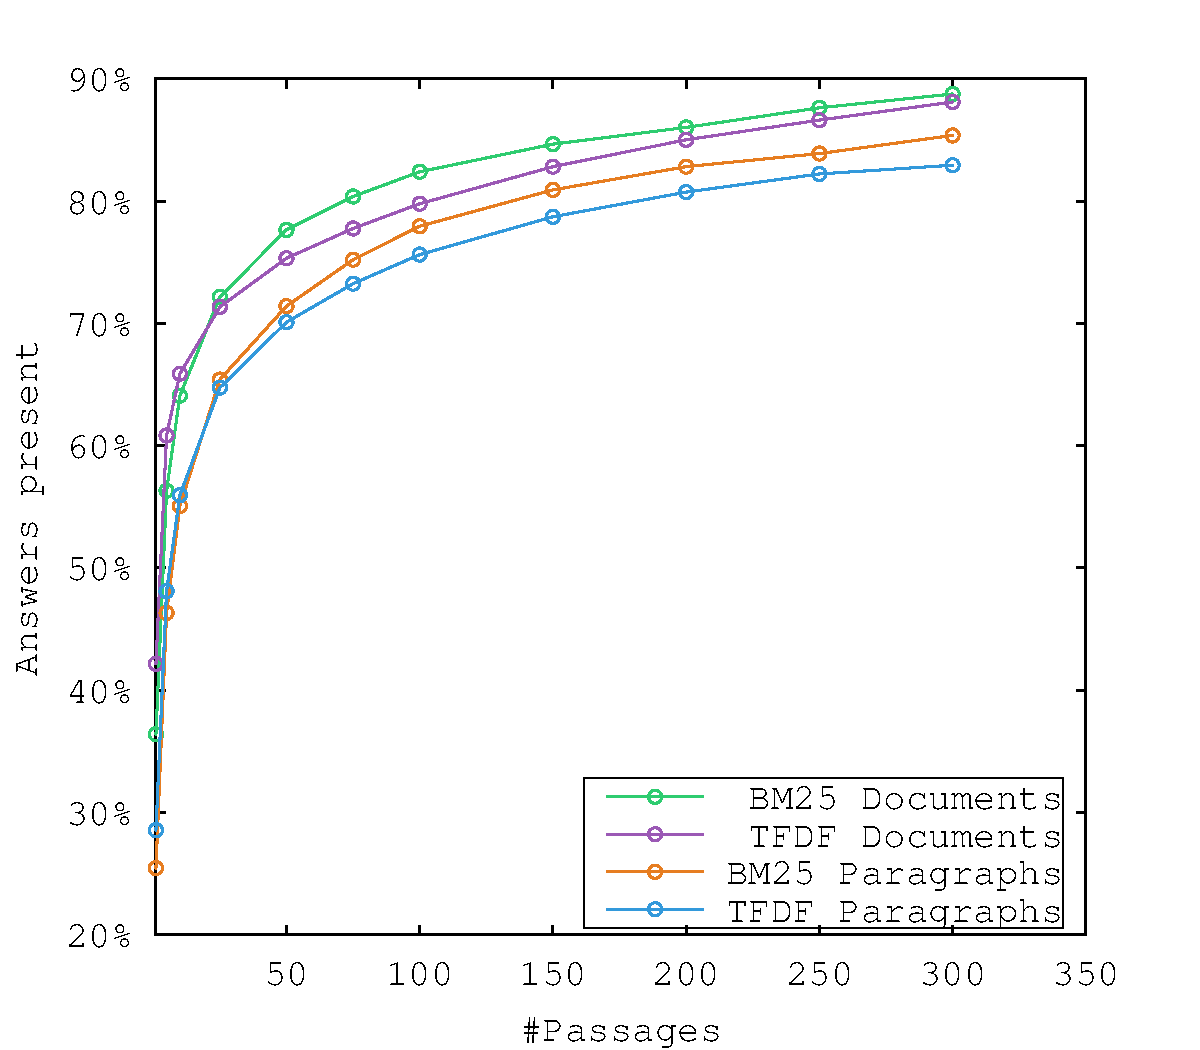
\includegraphics[width=0.5\textwidth]{figures/bm25_tfdf.pdf}
  \caption{Comparison between Lucene default, and BM25 similarities, when indexing by articles and paragraphs. 
  Shows how many percentages of the answers that were present for different number of passages.}
  \label{fig:bm25_tfdf}
\end{figure}

As we can see, BM25 is slightly better than Lucene default on all test with more than 25 passages, and no result can be 
considered acceptable using less than 25 passages.
Not surprisingly indexing by entire articles gives a better result than paragraphs, 
this can be explained by the fact that every article contains one or more paragraph. 
Which means that 100 article passages might yield the same amount of data as 200 paragraph passages.

\subsection{Noun extraction}

We needed to decide if we should index our wikipedia database dump by articles or paragraphs.
To decide this, we queried our two indexes, one indexed by paragraphs and
one indexed by articles, with all questions in our training set. We then extracted and 
ordered all nouns by frequency, and calculated the mean reciprocal rank.
If the answer was not present amongst the results, we disregarded the data point.

\begin{figure}[h!]
  \centering
  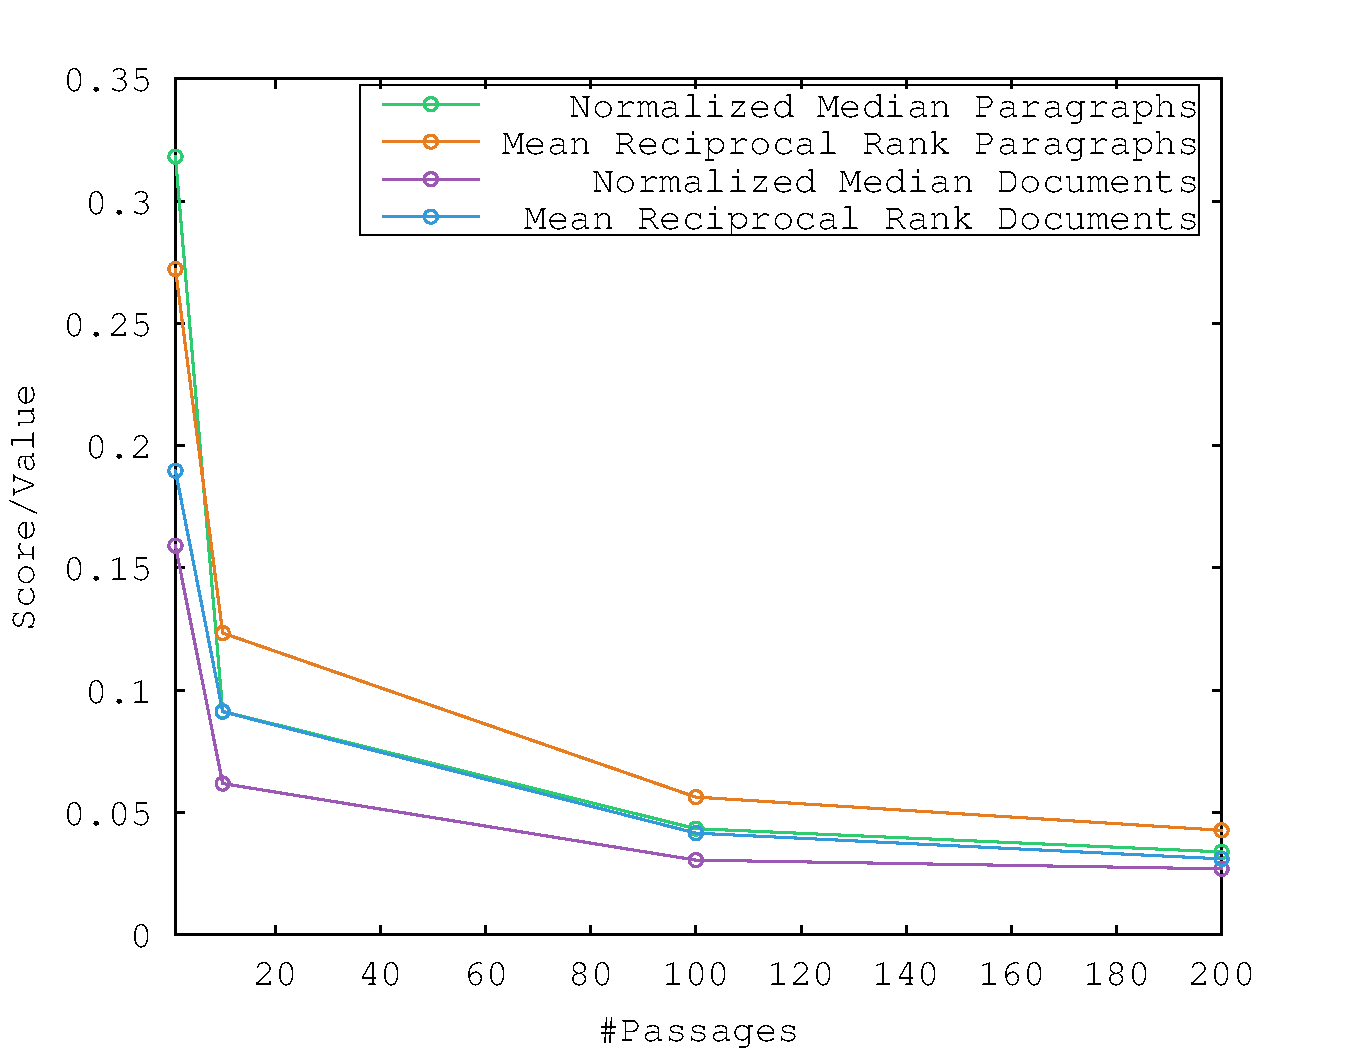
\includegraphics[width=0.5\textwidth]{figures/median.pdf}
  \caption{Comparison between indexing by articles, and indexing by paragraphs. 
  Shows the MRR values for the rank of the correct answer for the questions where 
  the answer is present.}
\end{figure}

As you can see, the mean reciprocal rank becomes lower as we extract more passages from the query, which
is natural since the frequency of frequently used swedish words increases as you increase the number
of passages extracted. Another phenomenon which we can observe is that the MRR for 
paragraphs is consistently higher than the MRR for documents, this is due to the amount of irrelevant
information contained in documents. Thus, the amount of relevant information is always more dense when
using a database indexed by paragraphs.

\subsection{Reranking}
Just extracting all nouns from the passages is not enough to acquire a valid answer, this is where the reranking comes in.
Using the trained model from all the questions, Liblinear is able to predict a probability that a specific noun is correct.
Combining this value with the value from Lucene, as mentioned, would increase the score of valid answers, and decrease the score of invalid ones.

Also, after reranking the answer candidates, there still exists some candidates that could be seen as impossible.
so using the puncher, as described, could in some cases improve the result further.

The result, measured using mean and median, can be seen in figure~\ref{fig:meanmedian}

\begin{figure}[h!]
  \centering
  \hspace*{-0.6cm}
  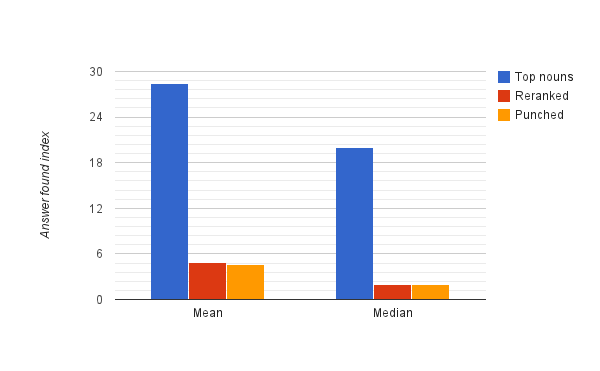
\includegraphics[width=0.6\textwidth]{figures/meanMedian.png}
  \caption{Comparison of answer ranks in the different stages of answer extraction.}
  \label{fig:meanmedian}
\end{figure}

The result, measured using MRR, can be seen in figure~\ref{fig:mrr}
\begin{figure}[h!]
  \centering
  \hspace*{-0.6cm}
  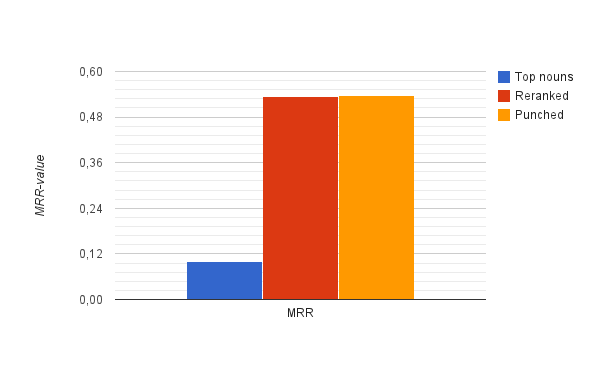
\includegraphics[width=0.6\textwidth]{figures/mrr.png}
  \caption{Comparison of answer ranks using MRR in the different stages of answer extraction.}
  \label{fig:mrr}
\end{figure}

As we can see, the reranking improves the result significantly, and the puncher gives a small boost.
By looking at the median values, we can see that for all the answers that are present, 
in half the cases the answer is located at the first or second place.


\begin{thebibliography}{}

\bibitem[\protect\citename{Aho and Ullman}1972]{Aho:72}
Alfred~V. Aho and Jeffrey~D. Ullman.
\newblock 1972.
\newblock {\em The Theory of Parsing, Translation and Compiling}, volume~1.
\newblock Prentice-{Hall}, Englewood Cliffs, NJ.

\bibitem[\protect\citename{{American Psychological Association}}1983]{APA:83}
{American Psychological Association}.
\newblock 1983.
\newblock {\em Publications Manual}.
\newblock American Psychological Association, Washington, DC.

\bibitem[\protect\citename{{Association for Computing Machinery}}1983]{ACM:83}
{Association for Computing Machinery}.
\newblock 1983.
\newblock {\em Computing Reviews}, 24(11):503--512.

\bibitem[\protect\citename{Chandra \bgroup et al.\egroup }1981]{Chandra:81}
Ashok~K. Chandra, Dexter~C. Kozen, and Larry~J. Stockmeyer.
\newblock 1981.
\newblock Alternation.
\newblock {\em Journal of the Association for Computing Machinery},
  28(1):114--133.

\bibitem[\protect\citename{Gusfield}1997]{Gusfield:97}
Dan Gusfield.
\newblock 1997.
\newblock {\em Algorithms on Strings, Trees and Sequences}.
\newblock Cambridge University Press, Cambridge, UK.

\end{thebibliography}

\end{document}
